\documentclass[a4paper]{article}

\usepackage[a4paper,  margin=1.0in]{geometry}

\usepackage{graphicx}
\usepackage{float}
\usepackage{hyperref}




\usepackage{polski}
\usepackage[utf8]{inputenc}
\begin{document}


\title{Laboratorium Rozpoznawania Obrazów – Ćwiczenie \#2 Klasyfikacja optymalna Bayesa}

\author{Michał Sypetkowski}
\maketitle


\section{Dane i ogólne uwagi}
Rozpatrujemy zbiór obrazów kart reprezentowanych przez niezmienniki momentowe.
Jest 8 klas, za równo w zbiorze trenującym i testującym jest wstępnie po 228 próbek na każdą klasę.

W eksperymentach rozpatrywane są 3 metody estymacji pdf:
\begin{enumerate}
\item Przy założeniu, że cechy są niezależne, a rozkłady każdej cechy są normalne (w tym
    przypadku gęstość prawdopodobieństwa dla więcej niż jednej cechy jest liczona jako
    iloczyn gęstości dla poszczególnych cech).
\item Przy założeniu, że mamy do czynienia z wielowymiarowym rozkładem normalnym dla cech
    używanych do klasyfikacji.
\item Przy użyciu okna Parzena do wyznaczenia aproksymacji gęstości prawdopodobieństwa na
    podstawie zbioru uczącego
    W eksperymentach innych niż \ref{parzen} przyjęta szerokość okna $h_1=0.001$.
\end{enumerate}

\section{Filtrowanie wartości odstających}
Algorytm filtrowania działa na danych znormalizowanych.
Dane są filtrowane poprzez odrzucenie próbek,
których wartość którejkolwiek cechy jest mniejsza
od kwartyla w 0.25 lub większa od kwartyla w 0.75 o 90 krotność odległości pomiędzy tymi kwartylami.
Implementacja jest w pliku \texttt{filter\_outliers.m}.

Ze zbioru trenującego odrzucona została próbka:
\begin{verbatim}
3.0000e+00 5.1213e+00 2.5823e+01 3.8214e+02 3.8086e+02 1.4530e+05 1.9341e+03 1.6570e+01
\end{verbatim}

Ze zbioru testującego próbki:
\begin{verbatim}
3.0000e+00 1.4815e-01 5.4870e-03 2.5403e-03 1.0161e-04 -5.1623e-08 -7.5267e-06 -1.7798e-16
3.0000e+00 1.4815e-01 5.4870e-03 2.5403e-03 1.0161e-04 -5.1623e-08 -7.5267e-06 -4.9372e-16
\end{verbatim}





\section{Optymalny klasyfikator Bayesa na 2 cechach}
Przyglądając się wizualizacji (rysunek \ref{fig:2D}) można dostrzec,
że kolumny 2 i 4 (kolumna 1 to klasa) zapewniają dość dobre oddzielenie próbek różnych klas.
Przeprowadziłem eksperyment polegający na posortowaniu wizualnie kilku par od najgorszych do najlepszych,
następnie sprawdziłem czy intuicja się zgadza, okazało się że tak
(poniżej wyniki dla klasyfikatorów używających 3 metod estymacji pdf).

\begin{verbatim}
run_on_features(train, test, [6 8]) % visually bad
   0.40176   0.40176   0.57300

run_on_features(train, test, [4 8]) % visually better
   0.22942   0.23216   0.26839

run_on_features(train, test, [4 5]) % ...
   0.15642   0.14599   0.23875

run_on_features(train, test, [2 4]) % visually best
   0.0246981   0.0038419   0.0230516

run_on_features(train, test, [2 3 4 5 6 7 8]) % all features
   0.0192097   0.0043908   0.0060373
\end{verbatim}
\begin{figure}[h]
    \caption[]{Wizualizacje 2D próbek zbioru uczącego dla wszystkich par cech}
    \centering
    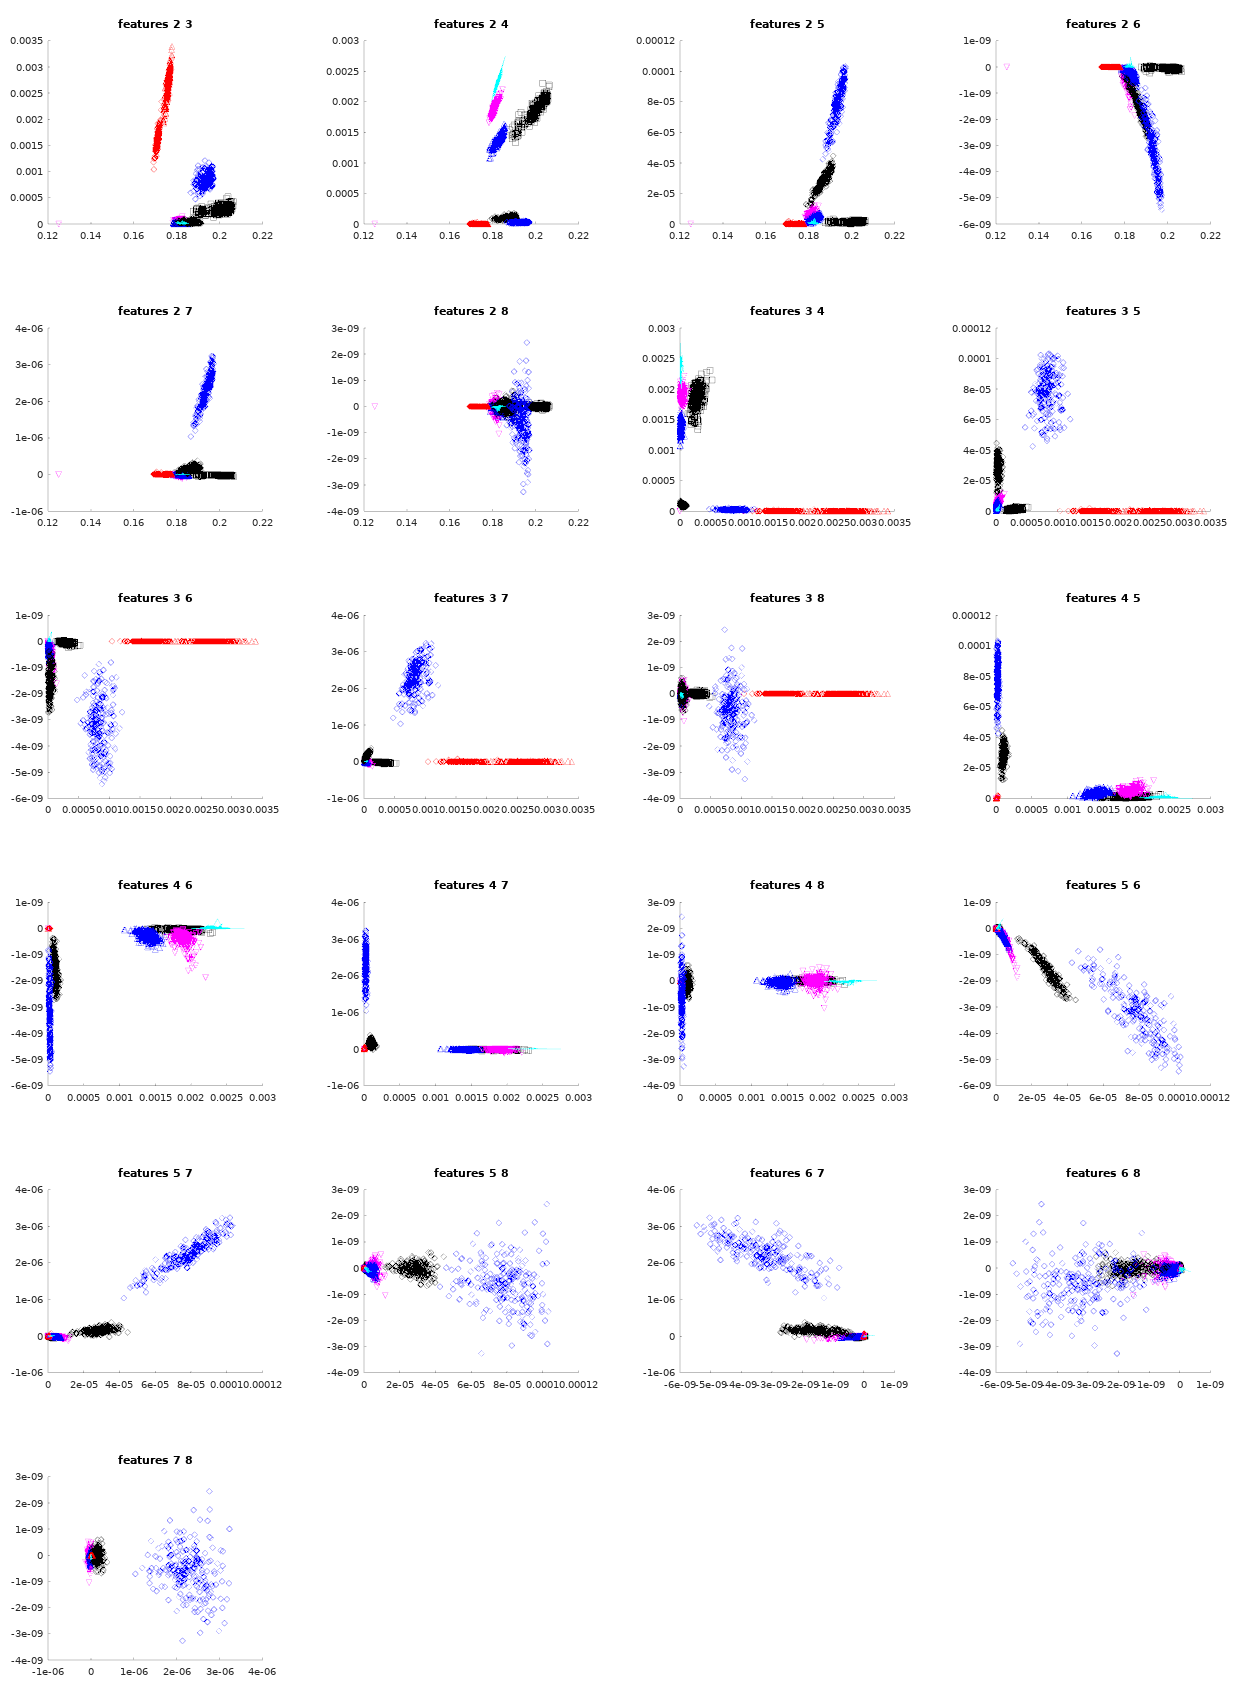
\includegraphics[width=1.0\textwidth]{2features.png}
    \label{fig:2D}
\end{figure}


\section{Wpływ doboru próbek w zbiorze uczącym na jakość klasyfikacji}\label{reduce}

Ten eksperyment bada wpływ na klasyfikację zbioru testowego, ma dobór próbek w zbiorze
uczącym (losowanie części próbek ze zbioru uczącego niezależnie dla poszczególnych klas).
Rysunek \ref{fig:reduce1} przedstawia wartość średnią pomiaru z odchyleniem standardowym.
Dla każdego współczynnika redukcji i dla każdego klasyfikatora eksperyment jest powtarzany po 20 razy.
Wykresy na rysunku \ref{fig:reduce2} "wyginają" się w górę wraz ze wzrostem współczynnika redukcji
(na wykresie liczności liczby próbek w wylosowanym podzbiorze).
Analogicznie maksima (rysunek \ref{fig:reduce3}) "wyginają" się w dół.
Wynika to z tego, że jest coraz mniej możliwości wylosowania podzbioru - w szczególności dla kompletnego zbioru wartość średnia, minimalna i maksymalna są równe,
a odcyhlenie standardowe jest równe 0.

Metoda estymacji pdf nr 1 sprawdza się dobrze tylko dla małych ilości próbek.
Metoda nr 2 sprawdza się ogólnie najlepiej, co świadczy o istnieniu korelacji między cechami (momentami obrazów).
Metoda nr 3 na małej ilości próbek sprawdza się najgorzej, ale dla dużej ilości dorównuje metodzie 2.
Można przypuszczać, że dla jeszcze większej ilości próbek ta metoda prześcignęła by metodę 2,
jednak jest znacząco gorsza wydajnościowo -- czas klasyfikacji rośnie w zależności od ilości próbek.

Można zaobserwować, ze estymacja z oknem Parzena wykazuje większą deterministyczność dla róznych podzbiorów próbek.
Odchylenia standardowe ma trochę mniejsze oraz kształt wykresu ma podobny
(a przynajmniej zachowuje monotonicznośc) dla średniej, minimum i maksimum.


\begin{figure}[h]
    \caption[]{Wpływ doboru próbek w zbiorze uczącym (zaznaczone odchylenie standardowe)}
    \centering
    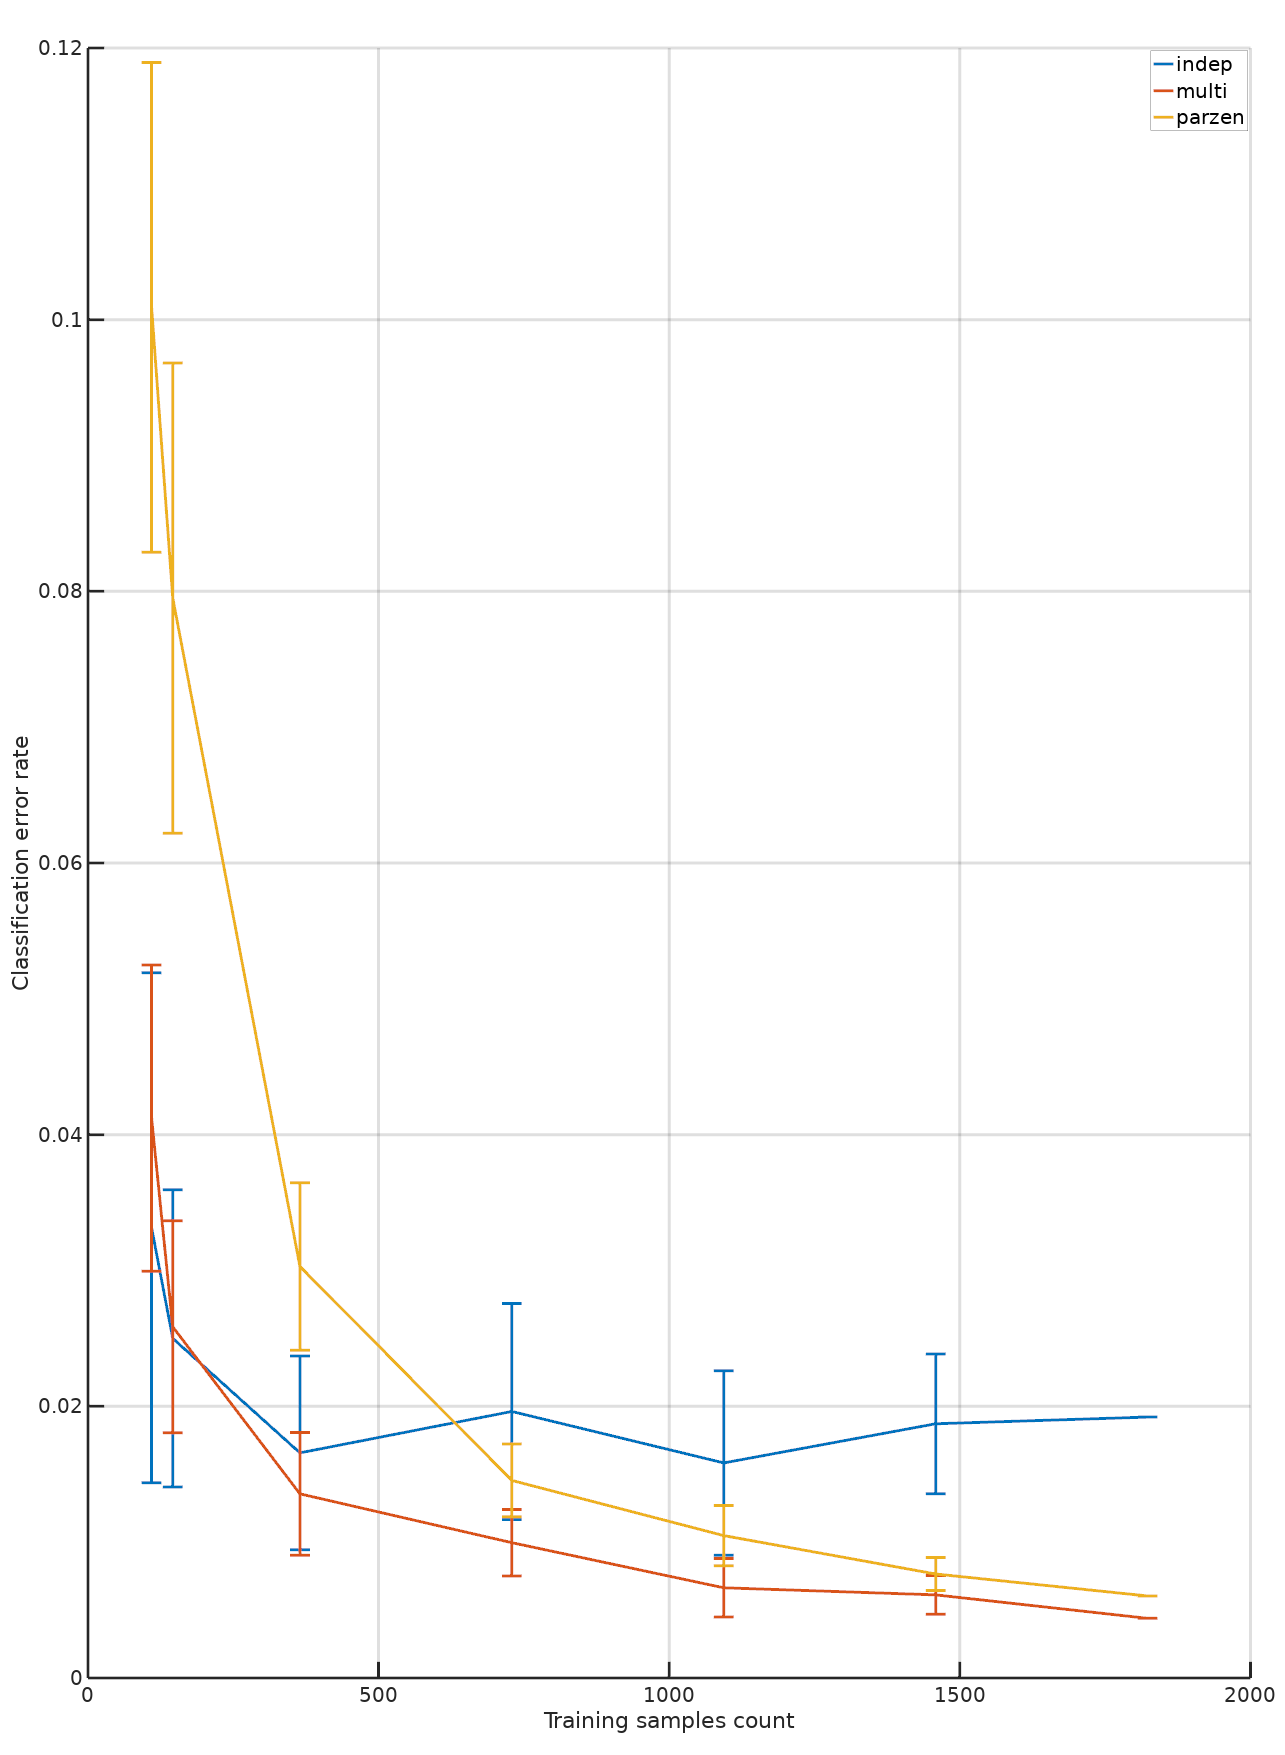
\includegraphics[width=1.0\textwidth]{reduce.png}
    \label{fig:reduce1}
\end{figure}

\begin{figure}[h]
    \caption[]{Wartość minimalna w każdym ekperymencie (patrz \ref{fig:reduce1})}
    \centering
    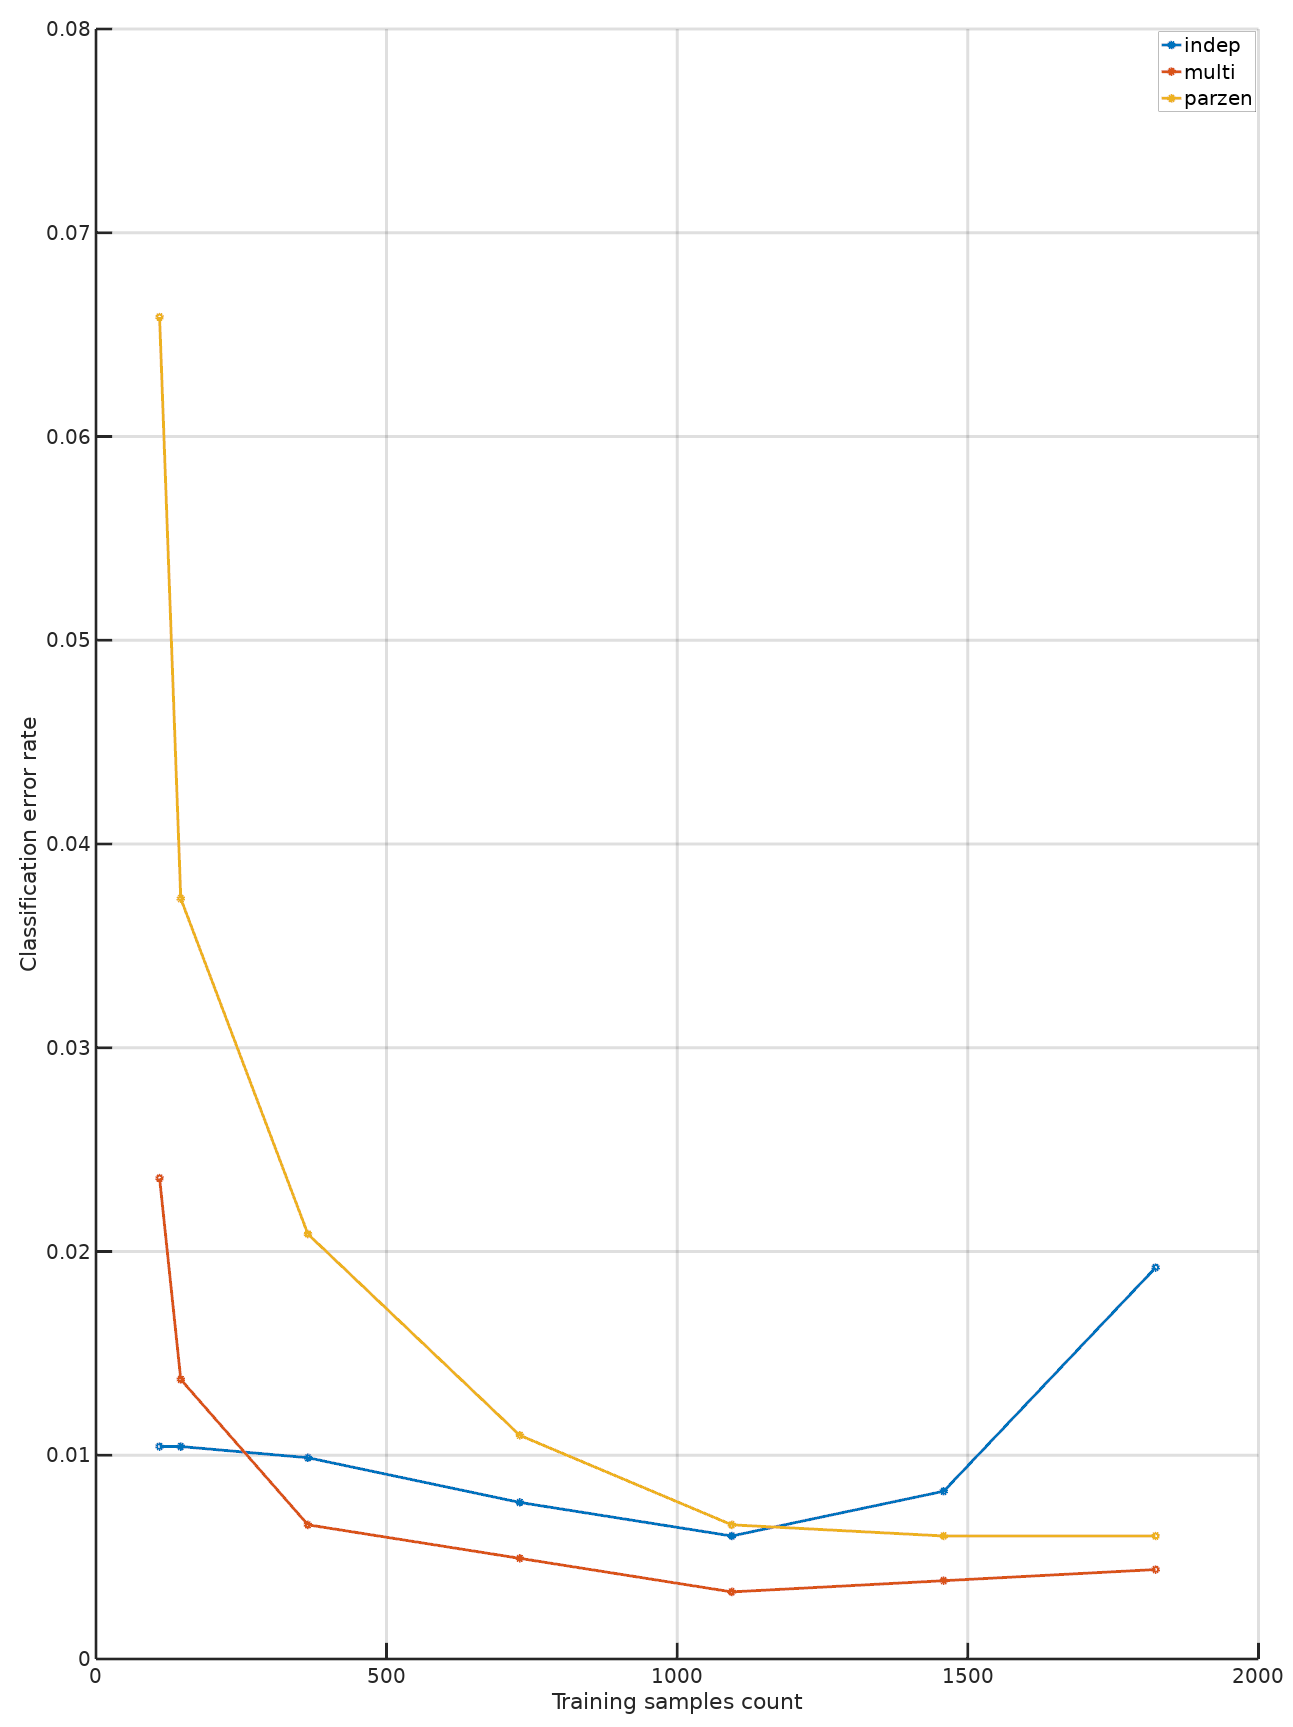
\includegraphics[width=1.0\textwidth]{reduceMin.png}
    \label{fig:reduce2}
\end{figure}

\begin{figure}[h]
    \caption[]{Podobnie jak w \ref{fig:reduce2}, tylko wartość maksymalna}
    \centering
    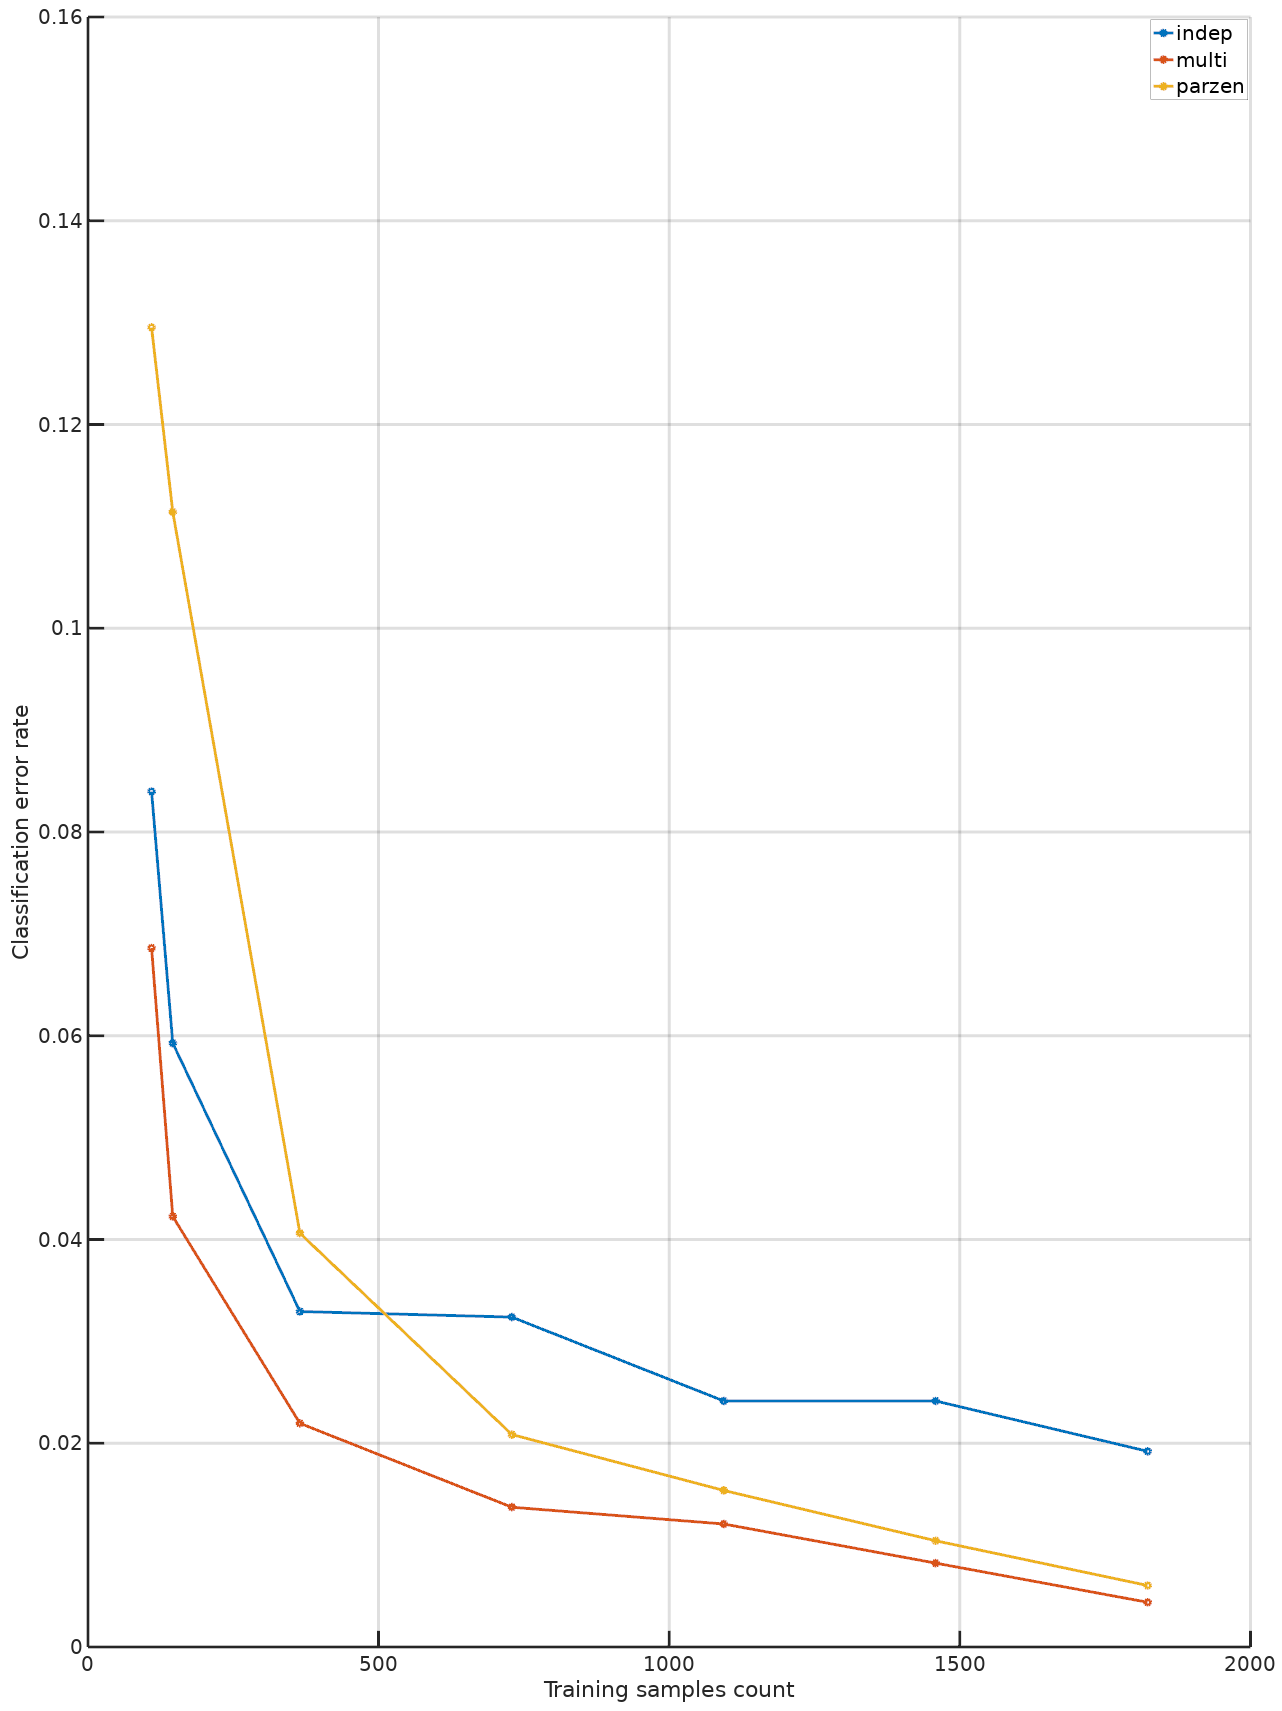
\includegraphics[width=1.0\textwidth]{reduceMax.png}
    \label{fig:reduce3}
\end{figure}

\section{Wpływ szerokości okna Parzena}\label{parzen}

Rysunek \ref{fig:window} pokazuje wartości średnie błędu klasyfikacji podobnie jak w eksperymencie \ref{reduce}.
Tutaj pozwolę sobie pominąć komentarz, bo wszystko widać na wykresie.
Pomiary są na podstawie 20 eksperymentów na każdy punkt na wykresie.

\begin{figure}[h]
    \caption[]{Wpływ doboru próbek w zbiorze uczącym (podobnie jak \ref{fig:reduce1}).
        Wartości średnie błędu na podstawie 20 eksperymentów.}
    \centering
    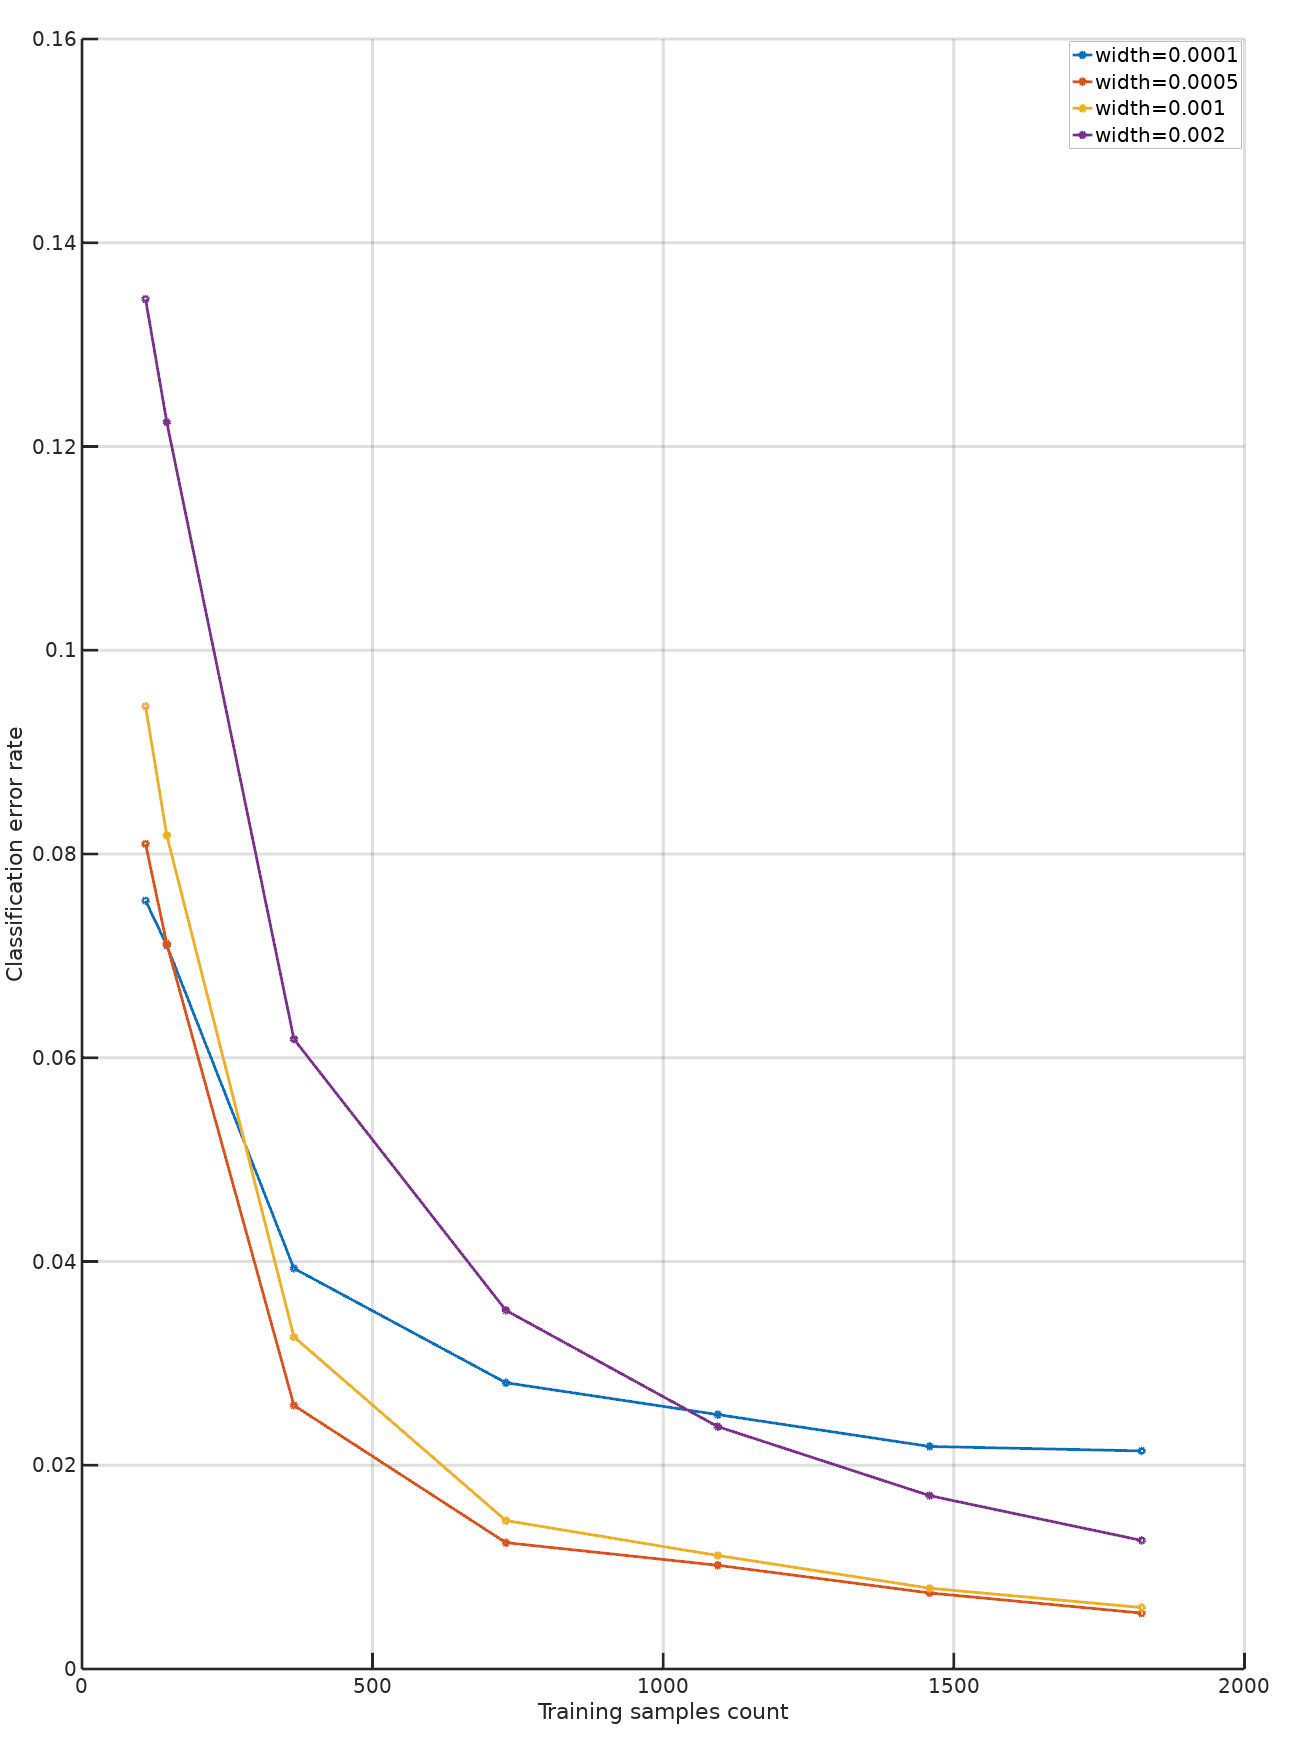
\includegraphics[width=1.0\textwidth]{window.png}
    \label{fig:window}
\end{figure}

\section{Eksperyment ze zmienionym prawdopodobieństwem a priori}
Zbiór testujący jest redukowany tak, że maści inne niż czerwone zamiast 228 próbek, mają po 114.
Poniższe pomiary uśredionych błędów są na podstawie 200 eksperymentów.
Uśredniony błąd klasyfikacji z poinformowaniem klasyfikatorów wektorem \texttt{[0.085 0.165 0.165 0.085 0.085 0.165 0.165 0.085]}:
\begin{verbatim}
0.0185286   0.0054905   0.0061713
\end{verbatim}
Uśredniony błąd klasyfikacji przy podaniu wektora z równymi elementami (\texttt{0.125}),
ale przy tak samo zredukowanym zbiorze testującym.
\begin{verbatim}
 0.0176318   0.0054941   0.0062811
\end{verbatim}
Dla porównania, wyniki dla całego zbioru z równymi a priori:
\begin{verbatim}
0.0192097   0.0043908   0.0060373
\end{verbatim}
Ogólnie, redukcja zbioru testującego spowodowała drobne pogorszenie wyników dla metody estymacji 1,
i drobne polepszenie wyników dla metod 2 i 3.
Informowanie klasyfikatorów o prawdopodobieństwach a priori ma bardzo mały wpływ na ich jakość.


\section{Porównanie z klasyfikatorem 1-NN}
TODO


\end{document}
